\lysh{37168}{2}

\begin{alist}
\item Το τριώνυμο $-x^2 + 5x - 6$ έχει $\alpha = -1, \beta = 5, \gamma = -6$ και διακρίνουσα:
\[\Delta = \beta^2 - 4\alpha\gamma = 5^2 - 4 \cdot (-1) \cdot (-6) = 25 - 24 = 1 > 0.\]

Οι ρίζες του τριωνύμου είναι οι:
\[x_{1,2} = \dfrac{-\beta \pm \sqrt{\Delta}}{2\alpha} = \dfrac{-5 \pm \sqrt{1}}{2 \cdot (-1)} = \begin{cases} 2 \\ 3 \end{cases}\]

Το πρόσημο του τριωνύμου φαίνεται στον παρακάτω πίνακα:
\begin{center}
\begin{tikzpicture}
\tikzset{t style/.style = {style = dashed}}
\tkzTabInit[color,lgt=3,espcl=2,colorC = maincolor!40,
colorL = maincolor!20,
colorV = maincolor!40]%
{$x$ / .8,$-x^2 +5x -6$ /0.8}%
{$-\infty$,$2$,$3$,$+\infty$}%
\tkzTabLine{ , $-$, z
, $+$ , z
, $-$ , }
\end{tikzpicture}
\end{center}

Επομένως ισχύει:
\[-x^2 + 5x - 6 < 0 \Leftrightarrow (x < 2 \text{ ή } x > 3) \Leftrightarrow x \in (-\infty, 2) \cup (3, +\infty).\]

Για την ανίσωση $x^2 - 16 \le 0$ ισχύει ότι:
\[x^2 - 16 \le 0 \Leftrightarrow x^2 \le 16 \Leftrightarrow \sqrt{x^2} \le \sqrt{16} \Leftrightarrow |x| \le 4 \Leftrightarrow -4 \le x \le 4 \Leftrightarrow x \in [-4, 4].\]

\item Αναπαριστούμε τις λύσεις των παραπάνω ανισώσεων στον ίδιο άξονα αριθμών.

Οι κοινές λύσεις των δύο ανισώσεων είναι:
\[-4 \le x < 2 \text{ ή } 3 < x \le 4 \Leftrightarrow x \in [-4, 2) \cup (3, 4].\]
\end{alist}
